% !TeX spellcheck = ru_RU
% !TEX root = vkr.tex

\section{Архитектура решения}

В данном разделе представлена реализация методов, упомянутых в обзорной части. В частности, алгоритм обхода в ширину с использованием параллельных вычислений и векторно-матричные операции.

\subsection{Детали реализации SpMSpV}

\begin{lstlisting}[style=fsharp, caption={Фрагмент функции сложения векторов, отвечающий за параллельную составляющую операции}, label={lst:add},  frame=single]
let vectorAddition level plusOperation vector1 vector2 =
   ...
   let rec treesAddition parallelLevel tree1 tree2 =
      match tree1, tree2 with
      ...
      | BinTree.Node (x, y), BinTree.Node (z, w) ->
         if parallelLevel = 0u then
            let left = treesAddition 0u x z
            let right = treesAddition 0u y w
            if left = BinTree.None && right = BinTree.None then
               BinTree.None
            else
               BinTree.Node(left, right)
         else
            let tasks =
                [| async { return treesAddition (parallelLevel - 1u) x z }; 
                   async { return treesAddition (parallelLevel - 1u) y w } |]
            let results = tasks |> Async.Parallel |> Async.RunSynchronously
\end{lstlisting}

На платформе .NET существует поддержка параллельных вычислений с использованием асинхронных (т.~e не блокирующих выполнение других процессов) выражений \texttt{async}, позволяющих разбить работу программы на небольшие подзадачи и запустить их параллельно на доступных вычислительных ядрах. Именно они были использованы при реализации векторно-матричных операций на языке F\#\footnote{Полная реализация алгоритма обхода в ширину и матрично-векторных операций: \url{https://github.com/PolinaSavelyeva/ProgrammingHomeworkFs}.}.

\newpage

Так как эффективность параллельной версии алгоритма, главным образом, зависит от количества используемых потоков, для векторно-матричных операций были добавлены параметры \texttt{level} --- для сложения и \texttt{multiLevel}, \texttt{addLevel} --- для умножения. Эти аргументы представляют собой \textit{уровни распараллеливания}; к примеру, для ненулевого \texttt{level} функции \texttt{vectorAddition} (лист. \ref{lst:add}) формируются две задачи, исполняемые параллельно,  для ненулевого \texttt{level} --- 1 формируются ещё две подзадачи и т.~д.

Аналогично сложению используются \texttt{multiLevel}, \texttt{addLevel} в функции \texttt{multi\-plication}, однако в процессе формируются четыре подзадачи вместо двух (лист. \ref{lst:multi}). Это различие обусловлено строением вектора и матрицы: узлы дерева, представляющего вектор, имеют ровно два потомка, а узлы дерева, представляющие матрицу --- четыре. 



\begin{lstlisting}[style=fsharp, caption={Фрагмент функции умножения вектора и матрицы, отвечающий за параллельную составляющую операции}, label={lst:multi},  frame=single]
let multiplication multiLevel addLevel fPlus fMulti vector matrix =
   if parallelLevel = 0u then
   ...
   else
     let multiTasks =
       [| async { return Vector(multiTrees (parallelLevel - 1u) left first,
                  vector.Length) }
          async { return Vector(multiTrees (parallelLevel - 1u) right third,
                  vector.Length) }
          async { return Vector(multiTrees (parallelLevel - 1u) left second,
                  vector.Length) }
          async { return Vector(multiTrees (parallelLevel - 1u) right fourth,
                  vector.Length) } |]
     let multiResults = multiTasks |> Async.Parallel |> Async.RunSynchronously
     let leftTree1 = multiResults[0]
     ...
     let addTasks =
       [| async { return (vectorAddition addLevel fPlus leftTree1 leftTree2).Storage }; async { return (vectorAddition addLevel fPlus rightTree1
       rightTree2).Storage } |]
     let addResults = addTasks |> Async.Parallel |> Async.RunSynchronously

\end{lstlisting}

\begin{figure}
    \centering
    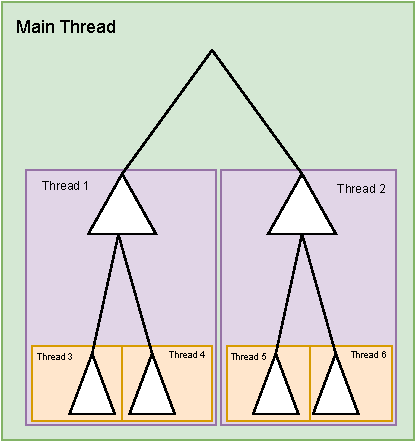
\includegraphics[width=0.6\textwidth]{QuadTree.pdf}
    \caption{Распределение потоков между узлами дерева, представляющего разреженный вектор, при сложении векторов (первый вектор отмечен синим цветом, второй красным)\\}
    \label{fig:tree}
    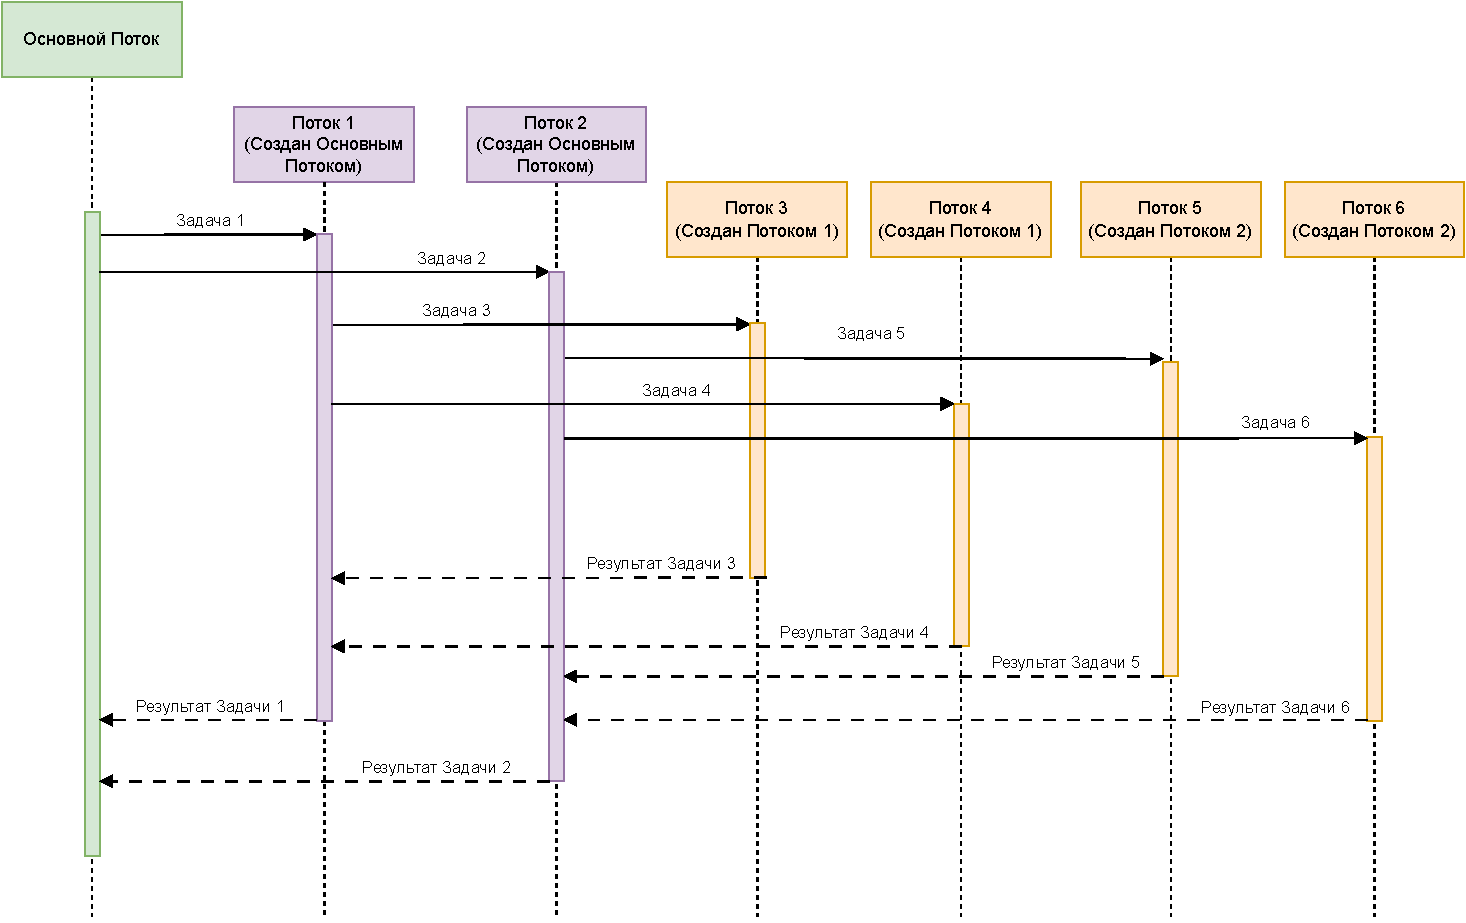
\includegraphics[width=0.9\textwidth]{SequentialUML.pdf}
    \caption{Последовательность выполнения операции сложения векторов с использованием многопоточности}
    \label{fig:uml}
\end{figure}

Визуализация распределения задач между узлами вектора при сложении представлена на рис. \ref{fig:tree}, а последовательность выполнения операции --- на рис. \ref{fig:uml}.

\subsection{Реализация BFS}

\begin{lstlisting}[style=fsharp, caption={Функция, реализующая обход в ширину с применением матрично-векторных операций}, label={lst:bfs},  frame=single]
let BFS multiLevel addMultiLevel addLevel startVertexList graph =
   let rec inner (front: Vector<unit>) visited iterationNumber =
      if front.IsEmpty then
         visited
      else
         let newFront = multiplication multiLevel addMultiLevel fPlus fMulti front graph.AdjacencyMatrix
         let front = vectorAddition addLevel fPlusMask newFront visited
         let visited = vectorAddition addLevel (fPlusVisited iterationNumber) visited front
         inner front visited (iterationNumber + 1u)
    let front = Vector(startVertexList, graph.VerticesCount, ())
    let visited = Vector(startVertexList, graph.VerticesCount, 0u)
    inner front visited 1u
\end{lstlisting}

Алгоритм BFS на лист. \ref{lst:bfs} реализует шаги 1--4, упомянутые в обзоре. Неочевидным остаётся шаг получения маски; в действительности необходимые действия выполняются в строке 7 без инициализации самой \texttt{mask}. Функция \texttt{fPlusMask} (лист. \ref{lst:mask}) используется при сложении нового фронта и вектора посещённых вершин --- на месте \texttt{front} получается ненулевое значение, только когда вершину предстоит посетить. 



\begin{lstlisting}[style=fsharp, caption={Функция, имитирующая поведение маски для обновления вектора-фронта}, label={lst:mask},  frame=single]
let fPlusMask a b =
    match a, b with
    | Some _, Option.None -> Some()
    | _ -> Option.None
\end{lstlisting}

